\section{Coupled Model Intercomparison Project 5 (CMIP5)}

\begin{frame} \frametitle{CMIP5 Models} { \fontsize{13pt}{14}\selectfont	

\begin{itemize} \setlength\itemsep{10pt}

    \item<1-> Set di dati multi-modello progettato per aumentare la nostra conoscenza del clima, la sua variabilità e il suo cambiamento attraverso l'applicazione di \textbf{GCMs} (General Circulation Models):
    \item<2-> Rispondono a concentrazioni specifiche e variabili nel tempo di vari componenti atmosferici.
	\item<3-> Il CMIP5 rappresenta due grandi gruppi di esperimenti di modellazione del cambiamento climatico:
	\begin{itemize}
        \item<4-> {\fontsize{12pt}{14}\selectfont Integrazione a lungo termine.}
	       \begin{itemize}
	           \item \textbf{Esperimento storico} (1850-2005).
	           \item \textbf{Representative Concentration Pathway  RCP2.6, RCP4.5, RCP6.0 e RCP8.5} (2006-2100).
	       \end{itemize}
	    \item<4-> {\fontsize{12pt}{14}\selectfont Integrazione a breve termine (decadale).}
	\end{itemize}  
\end{itemize}
	
%\begin{alertblock}<6->{The data (passwords) can only be accessed if:}
% \begin{itemize}
%       \setlength\itemsep{0pt}
%	     \item<2-> SEcube™ device is connected
%	     \item<2-> Login pin is the correct one
%	     \item<2-> Key inside the device is the correct one.
%	   \end{itemize}
%\end{alertblock}	
}	
\end{frame}



\begin{frame}
 \begin{center}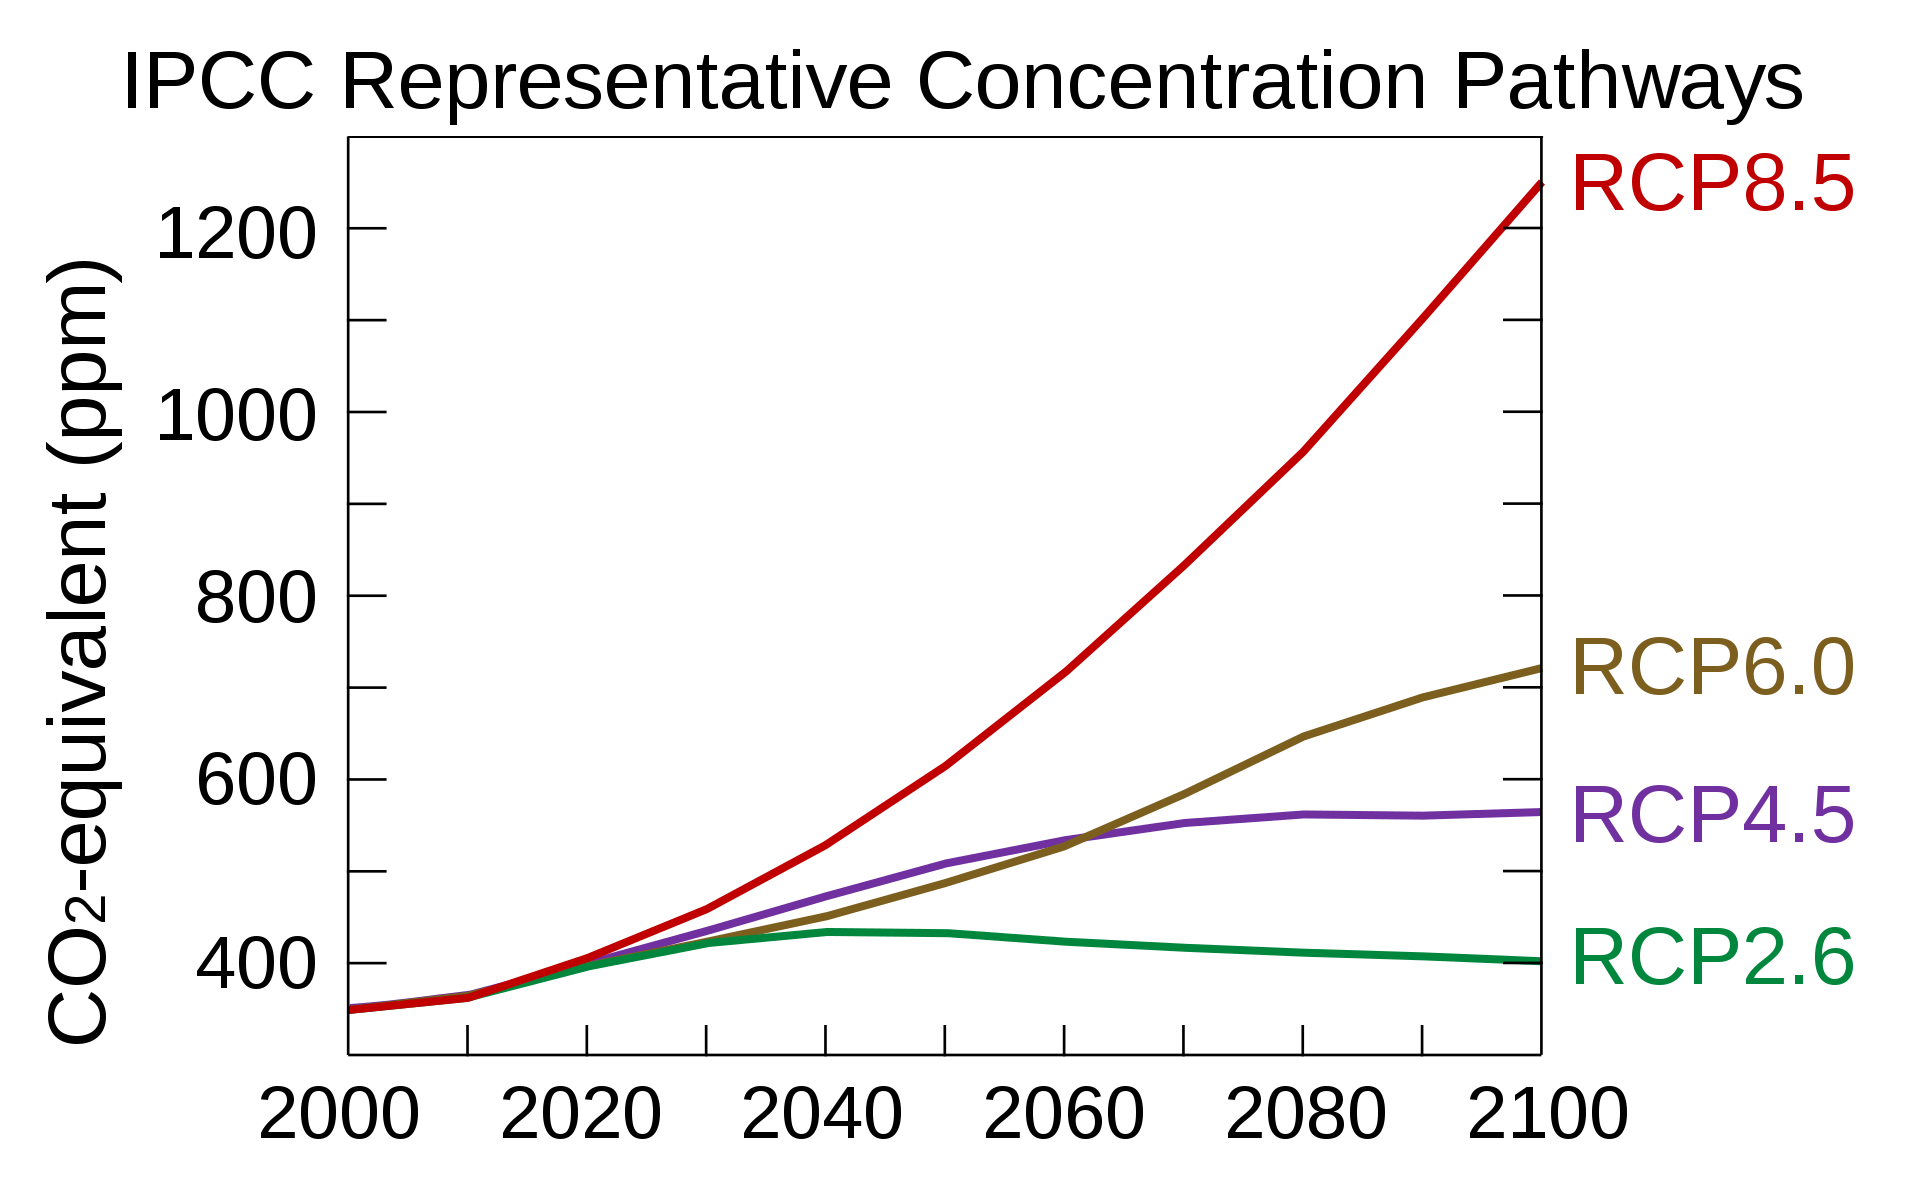
\includegraphics[width=\textwidth]{rcp}\end{center}
\end{frame}



\begin{frame}{pause}
      \frametitle{CMIP5 Models}
{\fontsize{10pt}{14}\selectfont

\centering
\begin{tabular}{lllcl}

\textbf{Variable}     &\textbf{Frequency}       &\textbf{Experiment}     & \textbf{N° Models}  & \textbf{Analysis}         \\ \hline
                                                                                                                           
pr                    & Daily                   & Historical             & $33$                  & ETCCDI Climate Indices    \\
                      &                         & RCP$4.5$               & $31$                  &                           \\
                      &                         & RCP$8.5$               & $33$                  &                           \pause \\
\hline                                                                                                                     
tasmin                & Daily                   & Historical             & $33$                  & ETCCDI Climate Indices    \\
                      &                         & RCP$4.5$               & $31$                  &                           \\
                      &                         & RCP$8.5$               & $33$                  &                           \\
\hline                                                                                                                     
tasmax                & Daily                   & Historical             & $34$                  & ETCCDI Climate Indices    \\
                      &                         & RCP$4.5$               & $32$                  &                           \\
                      &                         & RCP$8.5$               & $34$                  &                           \pause \\
                                                                                                                           
\hline                                                                                                                     
pr                    & Monthly                 & Historical             & $49$                  & Evaluation of models and  \\   
tas                   &                         & RCP$4.5$               & $45$                  & change in precipitation   \\
                      &                         & RCP$8.5$               & $42$                  & and temperature           \\

\end{tabular}
}
\end{frame}